\documentclass{../praktikum-protokollvorlage-latex/include/protokollclassE}
\SelectLanguage{english}

\input{../common/header.tex}

\newcommand{\versuch}{Lattice Vibration}
\newcommand{\betreuer}{Anna Steinig}
\newcommand{\durchgefuehrt}{08.01.18}

\newcommand{\abstract}{This report investigates the properties of oscillations inside a lattice based on the example of a mechanical model.
Values for various key parameters, such as the lattice parameter, strength of binding potentials (represented by the stiffness of springs), speed of sound, are given for a mono-/biatomic chain.
The measurements are carried out using a virtual instrument written in \texttt{LabView}.} %The abstract
\begin{document}
	\FrontMatter
	\include{titlepage.ag}
	\maketitlepage

	\MainMatter

	\chapter{Theory}
Small particles can be trapped in the focal point of a laser, held by radiation pressure.

Two models can be used to describe this effect, both depend on the laser beam having a gaussian intensity profile across its diameter.

\section{Geometrical Optics Model}
Geometrical optics only apply when the wavelength is much smaller than the feature size of the particles.
Also the particles are assumed to be roughly spherical.
In this case the laser beam can be split up into many parallel rays of light, which are refracted by the particles.
As the rays change direction at the boundaries, the photons transfer momentum to the particle, pushing it slightly towards the side where the ray hits the particle.
This is due to conservation of momentum, the photons leaving the particle have a different momentum than before entering the particle.
As the rays have lower intensities further away from the center of the beam, the force they impart on the particle is smaller and the particle experiences a net force towards the center of the beam.
\begin{figure}[bp]
  \centering
  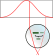
\includegraphics[width=.5\textwidth]{./img/geometrical-optics.pdf}
  \caption{Geometrical Optics Model}
\end{figure}

\section{Maxwell Model}
The above model only holds for large particles and small wavelengths.
For wavelengths that are of the same order as the particles themselves, a different model has to be considered.

The energy of a dielectric in an electric field is given by $U = -\vec{P}\vec{E}$.
For ''slow'' changing fields, the polarization is proportional to the electric field.
This results in an interaction energy of $U = -\Xi \vec{E}^2 \propto -I$ with the electric susceptibility $\Xi$ and the intensity of light $I$.

Due to the positive sign of $\Xi$ for small frequencies, the interaction energy of a particle in a beam with a gaussian intensity profile has a local minimum at the center, where intensity is highest.
The principle of minimum energy states that the particle lies in a stable state there. \todo{rephrase that}


\section{Brownian Motion}
If particles are suspended in a fluid, they perform random motions, namely \textbf{Brownian motion}, resulting from their collision with the thermal molecules inside the fluid.
Since the Brownian pattern is highly chaotic, probabilistic methods have to be employed to describe it.

Let $[t_\text{min}, t_\text{max}]$ be an interval during which the motion of a particle inside the fluid is tracked.
Let $t_0, t_1,\dots,t_n$ be a finite sequence of real numbers such that $t_\text{min}=t_0<t_1<\dots<t_n=t_\text{max}$.
If we determine the particle's location at each point of time in the partition, we may define the \textbf{mean square displacement (MSD)} as
\begin{equation}\label{eq:msd}
	r^2(t_i) = (x(t_i)-x(0))^2 + (y(t_i)-y(0))^2.
\end{equation}

Averaging these values over time yields the time-average MSD
\begin{equation}\label{eq:tamsd}
	\langle r^2 \rangle(t_n) = \frac{1}{n}\sum_{i=1}^n r^2(t_i),
\end{equation}
which can be adopted for multiple particles $m$
\begin{equation}\label{eq:mptamsd}
	\langle r^2 \rangle(t_n) = \frac{1}{m\cdot n}\sum_{j=1}^m\sum_{i=1}^n r^2_{i,j}(t_i).
\end{equation}

However, the MSD can be expressed in terms of the \textbf{diffusion coefficient} $D$,
\begin{equation}\label{eq:diff}
	\langle r^2 \rangle = 4Dt.
\end{equation}

Based on \textsc{Einstein}'s work \cite{einstein}, we may write $D$ like
\begin{equation}\label{eq:diff_einstein}
	D=\frac{k_\text{B}T}{6\pi\eta_\text{eff}a},
\end{equation}
where $\eta_\text{eff}$ denotes the viscocity of the fluid and $a$ is the particle radius.

Fitting the linear model in \autoref{eq:diff} to data yields a slope
\begin{equation*}
	m = \frac{D}{4}.
\end{equation*}

Rearraging this expression for $D$ and using \autoref{eq:diff_einstein} yields
\begin{equation}\label{eq:vis}
	\eta_\text{eff} = \frac{2k_\text{B}T}{3\pi ma}.
\end{equation}

\section{Maximum Trapping Force}
To determine the maximum trapping force $F_\text{trap,max}$, we shall assume that the particles flow laminarily.
Hence, the occuring friction force obeys \textsc{Stokes}'s law
\begin{equation*}
	F_\text{S} = 6\pi\cdot\eta_\text{eff}av.
\end{equation*}
The particle remains trapped if the condition
\begin{equation*}
	F_\text{trap,max} \stackrel{!}{=} F_\text{S}\rvert_{v_\text{max}} = \frac{4k_\text{B}T}{m}v_\text{max}
\end{equation*}
is satisfied.

Typical values of $F_\text{trap,max}$ are within the \si{\pico\newton}-range.

	% !TEX root = ../05-Lattice-Vibration.tex
\chapter{Procedure}
\section{Model}
The model consists of twelve thingimajigs and thirteen springs.
The first spring is connected to a stepper motor that can creates reciprocal harmonic motion at a selectable frequency and presents a fixed end to the chain.
The last spring is fixed to the end of the rail.

The thingimajigs consist of a piece of angle aluminum and have a threaded hole to mount additional weights.
Each thingimajig has a stripe of retroreflective material glued to it's side.
They ride on a linear air bearing which is a square tube sealed on both ends oriented on one of it's edges.
A turbine sends an air stream into the tube.
The tube's two sides facing upwards have a series of small holes to create an air cushion between the tube and the thingimajigs.
To dampen the oscillation after an experiment, the turbine's air inlet is blocked briefly.

\section{Data Aquisition}
A camera with a horizontal linear CCD is used to capture the position the retroreflective stripes on the fifth and sixth thingimajig.
Prior to the experiment the camera is aligned so the retroreflectors are in the plane of the CCD.
A \texttt{LabView} program is used to read the two positions from the camera.
The program is then used to apply a fast fourier transform to the positions to find the frequencies of the individual modes and later to measure the amplitudes of single modes.

	\chapter{Data}
\section{Dispersion Relations}

\subsection{''Monoatomic'' Chain}
\begin{figure}
	\centering
	\includegraphics[width=0.7\textwidth]{./data/plots/dispersion_single_data.pdf}
	\caption[Dispersion Relation of Monoatomic Chain]{\textbf{Dispersion Relation of Monoatomic Chain} Edge of first Brillouin zone is marked in green.
	Dispersion function $\omega(k) = \sqrt{\frac{4D}{m}}\abs{\sin\left(\frac{ka}{2}\right)}$ with known mass $m$ and lattice parameter $a$ is fitted to the data.
	Found fit parameter: $D=\SI{27.05(9)}{\newton\per\meter}$. Goodness of fit: $\chi_\text{red}=\num{0.003}$.}
	\label{fig:dispersion_single}
\end{figure}

\subsection{''Biatomic'' Chain}
\begin{figure}
	\centering
	\includegraphics[width=0.7\textwidth]{./data/plots/dispersion_alternating_data.pdf}
	\caption[Dispersion Relation of Biatomic Chain]{\textbf{Dispersion Relation of Biatomic Chain} Edge of first Brillouin zone is marked in green.
	Dispersion functions $\omega_{-}$ and $\omega_{+}$ discussed in \autoref{sec:alt_theory} with known masses $m$, $M$ and lattice parameter $a$ are fitted to the data.
	Found fit parameters: $D_\text{opt}=\SI{24.6(3)}{\newton\per\meter}, D_\text{ac}=\SI{21.7(3)}{\newton\per\meter}$. Goodness of fit: $\chi_\text{opt, red}=\num{0.028}, \chi_\text{ac, red}=\num{0.007}$.}
	\label{fig:dispersion_single}
\end{figure}

\section{Amplitude Ratio of hetherogenous linear Chain}
The amplitude ratio $\frac{s_{o,m}}{s_{o,M}}$ is determined for each mode of the model.
For obvious reasons the amplitudes $s_{o,m}$ and $s_{o,M}$ cannot be measured at the same location in the chain.
Instead, the amplitudes $A_{5/6}$ of the fifth and sixth thingamajig are measured using the camera system.
The fifth thingamajig has mass $M$, the sixth has mass $m$.
To obtain the actual amplitude ratio of the envelope functions, the ratio $\frac{A_{6}}{A_{5}}$ is multiplied with the ratio of the local amplitudes of the envelopes at position five and six:
\begin{equation*}
	\frac{s_{o,m}}{s_{o,M}} = \frac{A_{6}}{A_{5}} \cdot \frac{\sin(\frac{\uppi n}{13} \cdot 5)}{\sin(\frac{\uppi n}{13} \cdot 6)}.
\end{equation*}


\todo{probably put this table somewhere else}

\begin{table}
	\centering
	\caption[Amplitude Ratios of hetherogenous linear Chain:]{\textbf{Amplitude Ratio of hetherogenous linear Chain:} The amplitudes $A_n$ and $B_n$ of two thingamajigs (5th and 6th thingamajig) are measured. The ratio is corrected for the different position in the chain to obtain the correct amplitude ratio between heavy and light thingamajigs.}
	\begin{tabular}{SSSSS}
		\toprule
		{$n$}&
		{$f$ (\si{\hertz})}&
		{$A_{5,n}$}&
		{$A_{6,n}$}&
		{Corrected Ratio}\\
		\midrule
		1&	0.240&	 143.1 \pm  0.1&	 143.1 \pm  0.1&	+0.99 \pm 0.00\\
		2&	0.477&	  90.6 \pm  0.1&	  90.6 \pm  0.1&	+0.99 \pm 0.00\\
		3&	0.705&	  96.9 \pm  0.3&	  96.9 \pm  0.5&	+0.92 \pm 0.00\\
		4&	0.919&	 166.9 \pm  1.6&	 166.9 \pm  2.8&	+0.86 \pm 0.03\\
		5&	1.109&	  39.1 \pm  0.2&	  39.1 \pm  0.3&	+0.64 \pm 0.00\\
		6&	1.248&	 126.1 \pm  1.5&	 126.1 \pm  0.6&	+0.30 \pm 0.00\\
		7&	1.659&	  15.3 \pm  0.5&	  15.3 \pm  0.5&	-5.16 \pm 0.19\\
		8&	1.755&	   8.5 \pm  0.9&	   8.5 \pm  0.7&	-2.32 \pm 0.29\\
		9&	1.866&	  49.1 \pm  0.5&	  49.1 \pm  0.5&	-1.79 \pm 0.02\\
		10&	1.963&	  22.1 \pm  0.5&	  22.1 \pm  0.5&	-1.61 \pm 0.03\\
		11&	2.035&	  33.7 \pm  0.4&	  33.7 \pm  0.6&	-1.50 \pm 0.04\\
		12&	2.078&	  56.0 \pm  0.3&	  56.0 \pm  0.4&	-1.60 \pm 0.01\\
		\bottomrule
	\end{tabular}
\end{table}


	\Appendix
\configureappendix
\section{Data}
\setcounter{table}{0}
\def \hfillx {\hspace*{-\textwidth} \hfill}

\begin{table}[h]
	\caption{Eigenfrequencies: Monoatomic Chain, Series 1\&2}
	\label{tab:eigenfreq_a1_12a}
	\begin{tabular}{S|SS}
		\toprule
		{mode $n$}	&	{frequency $\omega_{n,\text{1}}$}	&	{frequency $\omega_{n,\text{2}}$} \\
		\midrule
		1	&	1.738	&	1.738	\\
		2	&	3.460	&	3.460	\\
		3	&	5.131	&	5.131	\\
		4	&	6.745	&	6.745	\\
		5	&	8.254	&	8.254	\\
		6	&	9.650	&	9.650	\\
		7	&	10.938	&	10.938	\\
		8	&	12.052	&	12.052	\\
		9	&	12.993	&	12.993	\\
		10	&	13.745	&	13.745	\\
		11	&	14.307	&	14.307	\\
		12	&	14.627	&	14.627	\\
		\bottomrule
	\end{tabular}
	\hfillx
	\begin{tabular}{S|SS}
		\toprule
		{mode $n$}	&	{frequency $\omega_{n,\text{1}}$}	&	{frequency $\omega_{n,\text{2}}$} \\
		\midrule
		1	&	1.740	&	1.740	\\
		2	&	3.456	&	3.456	\\
		3	&	5.130	&	5.130	\\
		4	&	6.733	&	6.733	\\
		5	&	8.246	&	8.246	\\
		6	&	9.643	&	9.643	\\
		7	&	10.927	&	10.927	\\
		8	&	12.039	&	12.039	\\
		9	&	12.979	&	12.979	\\
		10	&	13.734	&	13.734	\\
		11	&	14.299	&	14.299	\\
		12	&	14.613	&	14.613	\\
		\bottomrule
	\end{tabular}
\end{table}
\begin{table}[h]
	\caption{Eigenfrequencies: Monoatomic Chain, Series 3\&4}
	\label{tab:eigenfreq_a1_34a}
	\begin{tabular}{S|SS}
		\toprule
		{mode $n$}	&	{frequency $\omega_{n,\text{1}}$}	&	{frequency $\omega_{n,\text{2}}$} \\
		\midrule
		1	&	1.738	&	1.738	\\
		2	&	3.462	&	3.462	\\
		3	&	5.131	&	5.131	\\
		4	&	6.736	&	6.736	\\
		5	&	8.250	&	8.250	\\
		6	&	9.649	&	9.649	\\
		7	&	10.931	&	10.931	\\
		8	&	12.043	&	12.043	\\
		9	&	12.982	&	12.982	\\
		10	&	13.736	&	13.736	\\
		11	&	14.304	&	14.304	\\
		12	&	14.620	&	14.619	\\
		\bottomrule
	\end{tabular}
	\hfillx
	\begin{tabular}{S|SS}
		\toprule
		{mode $n$}	&	{frequency $\omega_{n,\text{1}}$}	&	{frequency $\omega_{n,\text{2}}$} \\
		\midrule
		1	&	1.742	&	1.742	\\
		2	&	3.460	&	3.460	\\
		3	&	5.134	&	5.134	\\
		4	&	6.739	&	6.739	\\
		5	&	8.252	&	8.252	\\
		6	&	9.647	&	9.647	\\
		7	&	10.929	&	10.930	\\
		8	&	12.050	&	12.050	\\
		9	&	12.985	&	12.985	\\
		10	&	13.745	&	13.745	\\
		11	&	14.306	&	14.306	\\
		12	&	14.620	&	14.621	\\
		\bottomrule
	\end{tabular}
\end{table}
\begin{table}[h]
	\caption{Eigenfrequencies: Biatomic Chain, Series 1\&2}
	\label{tab:eigenfreq_a1_12b}
	\begin{tabular}{S|SS}
		\toprule
		{excitation $n$}	&	{freq. $\omega_{n,\text{1}}$}	&	{freq. $\omega_{n,\text{2}}$} \\
		\midrule
		1	&	1.509	&	1.509	\\
		2	&	2.996	&	2.996	\\
		3	&	4.428	&	4.428	\\
		4	&	5.773	&	5.773	\\
		5	&	6.970	&	6.971	\\
		6	&	7.839	&	7.839	\\
		7	&	10.422	&	10.421	\\
		8	&	11.028	&	10.821	\\
		9	&	11.722	&	11.028	\\
		10	&	12.336	&	11.722	\\
		11	&	12.786	&	12.336	\\
		12	&	13.057	&	12.787	\\
		\bottomrule
	\end{tabular}
	\hfillx
	\begin{tabular}{S|SS}
		\toprule
		{excitation $n$}	&	{freq. $\omega_{n,\text{1}}$}	&	{freq. $\omega_{n,\text{2}}$} \\
		\midrule
		1	&	1.512	&	1.512	\\
		2	&	2.992	&	2.992	\\
		3	&	4.429	&	4.429	\\
		4	&	5.778	&	5.778	\\
		5	&	6.970	&	6.970	\\
		6	&	7.839	&	7.838	\\
		7	&	10.423	&	10.423	\\
		8	&	11.023	&	11.023	\\
		9	&	11.720	&	11.720	\\
		10	&	12.337	&	12.337	\\
		11	&	12.783	&	12.783	\\
		12	&	13.057	&	13.056	\\
		\bottomrule
	\end{tabular}
\end{table}
\begin{table}[h]
	\caption{Eigenfrequencies: Biatomic Chain, Series 3\&4}
	\label{tab:eigenfreq_a1_34b}
	\begin{tabular}{S|SS}
		\toprule
		{excitation $n$}	&	{freq. $\omega_{n,\text{1}}$}	&	{freq. $\omega_{n,\text{2}}$} \\
		\midrule
		1	&	1.509	&	1.509	\\
		2	&	2.997	&	2.997	\\
		3	&	4.427	&	4.427	\\
		4	&	5.778	&	5.778	\\
		5	&	6.974	&	6.974	\\
		6	&	7.840	&	7.840	\\
		7	&	10.426	&	10.426	\\
		8	&	11.030	&	11.030	\\
		9	&	11.723	&	11.723	\\
		10	&	12.334	&	12.334	\\
		11	&	12.783	&	12.783	\\
		12	&	13.057	&	13.057	\\
		\bottomrule
	\end{tabular}
	\hfillx
	\begin{tabular}{S|SS}
		\toprule
		{excitation $n$}	&	{freq. $\omega_{n,\text{1}}$}	&	{freq. $\omega_{n,\text{2}}$} \\
		\midrule
		1	&	1.513	&	1.513	\\
		2	&	2.998	&	2.998	\\
		3	&	4.429	&	4.429	\\
		4	&	5.775	&	5.775	\\
		5	&	6.975	&	6.975	\\
		6	&	7.840	&	7.840	\\
		7	&	10.427	&	10.427	\\
		8	&	11.027	&	11.027	\\
		9	&	11.728	&	11.728	\\
		10	&	12.337	&	12.337	\\
		11	&	12.790	&	12.790	\\
		12	&	13.060	&	13.060	\\
		\bottomrule
	\end{tabular}
\end{table}

	%\include{bibliography.ag}
\end{document}
